\begin{comment}
	Heuristica para ASV
	Introducción
	Cantidad de órdenes topológicos de un DAG
	Queremos topoSorts(polyTree) pues nuestra red es un polytree.
	Cantidad de ordenes topológicos para un “árbol”.
	Cantidad de clases de equivalencia para un “árbol”
\end{comment}


Recordemos la definición de la fórmula de ASV:

\begin{align*}
	\assym_{M,e,\Pr}(x_i) = \sum_{\pi \in \topo(G)} [\charactheristicFunction_{M,e,\Pr}(\pi_{<i} \cup \{x_i\}) - \charactheristicFunction_{M,e,\Pr}(\pi_{<i})] 
\end{align*}

Para simplificar la notación, tomemos $M,e$ y $Pr$ fijos, de modo que $\charactheristicFunction_{M,e,\Pr} = \charactheristicFunction$. La idea es encontrar un criterio para disminuir el número de órdenes topológicos que necesitamos calcular, reduciendo la cantidad de veces que evaluaremos $\charactheristicFunction$. La idea principal detrás de esta heurística es, identificar las clases de equivalencia para los diferentes órdenes topológicos $\toOr^1, \toOr^2 \in \topo(G)$, tales que $\toOr^1 \rel^\star \ \toOr^2 \iff \charactheristicFunction(\toOr^1_{<i}) = \charactheristicFunction(\toOr^2_{<i}) $. Nuestro algoritmo va a trabajar sobre una relación \rel{} más fina que $\rel^\star$, pues esta es costosa de calcular. Al conjunto de clases de equivalencia de $G$ definido por la relación \rel{} lo vamos a denotar como $eqCl(G, x_i)$. Una vez que consigamos todas las clases de equivalencia $\equivalenceClass$, solo necesitamos un representante de cada una y su tamaño para calcular el ASV:

\begin{align*}
	&\assym_{M,e,\Pr}(x_i)\\
	&= \frac{1}{\topo(G)} \sum_{\toOr \in \topo(G)} \charactheristicFunction(\toOr_{<i} \cup \{x_i\}) - \charactheristicFunction(\toOr_{<i}) \\
	&=  \heuristicASVFormula
\end{align*}

%\santi{Por qué $R'$ y no $R$?} \echu{Porque $R$ es la relación "posta" que definimos más adelante, entonces para la que es la ideal use $R'$. Tal vez le podría poner otro nombre, tipo $I$, porque es raro meter un $'$ de la nada. }

%\santi{Ah, entiendo. Capaz pondría $R$ a esta y a la otra $R^\star$, porque el prima acá es raro. Adelantaría en este punto que nuestro algoritmo va a trabajar sobre una clase más fina que esta $R'$ porque no es fácil calcularla} Rta: Todo el sentido del mundo

%Usando nuestra nueva fórmula, las permutaciones que estudiaremos son las de $topo(G)$. Ahora nos vamos a centrar en las clases de equivalencia de $\topo(G)$ siguiendo los criterios definidos anteriormente, teniendo en cuenta que estamos calculando $\phi_{i}^{assym}(\charactheristicFunction)$. \santi{No entiendo a que van estas primeras dos oraciones} $$ Rta: No suman mucha info, las sacamos

\begin{figure}[ht]
	\centering 
	\begin{tikzpicture}[scale=.95, transform shape]
		
		% ---- NODOS ----
		\node[nodo] (a1) at (0, 0) {$a_1$};
		\node[nodo] (a2) at (2.5, 2) {$a_2$};
		\node[nodo] (a3) at (2.5, -2) {$a_3$};
		\node[nodo] (xi) at (5, 0) {$x_i$};
		\node[nodo] (d_1) at (7.5, 2) {$d_1$};
		\node[nodo] (d_2) at (10, -2) {$d_2$};
		\node[nodo] (d_3) at (10, 0) {$d_3$};
		
		\node[draw=none, fill=none] (hijo_a3) at (4.5, -4) {};
		\node[draw=none, fill=none] (hijo_d2) at (8, -4) {};
		
		% ---- ARISTAS ----
		\path [->] (a1) edge[arista, mySnake]  (xi);
		\path [->] (a2) edge[arista, mySnake]  (xi);
		\path [->] (a3) edge[arista, mySnake]  (xi);
		\path [->] (xi) edge[arista, mySnake]  (d_1);
		\path [->] (xi) edge[arista, mySnake]  (d_2);
		\path [->] (xi) edge[arista, mySnake]  (d_3);
		\path [->] (a3) edge[arista, mySnake] node[above right] {descendientes de $a_3$ } (hijo_a3);
		\path [->] (hijo_d2) edge[arista, mySnake] node[below right] {ancestros de $d_2$ } (d_2);
		
	\end{tikzpicture}
	\caption{Al fijar un nodo $x_i$, podemos dividir el resto de los nodos en tres grupos: \textit{ancestros} (todos los nodos que pueden alcanzar a $x_i$), \textit{descendientes} (todos los nodos alcanzables desde $x_i$) y aquellos \textit{no relacionados} con $x_i$. Los \textit{no relacionados} son los que no pertenecen a los ancestros ni a los descendientes, por lo que pueden estar a la derecha o la izquierda de $x_i$ en un orden topológico.}
	\label{fig:unrelatedNodesDefinition}
\end{figure}

%\sergio{Puse en tesis.tex el package caption para hacer que las captions sean más chicas, y así más distinguibles del texto principal. Se puede cambiar}

Sea nuestro DAG $G=(V,E)$, con $A$ el conjunto de ancestros de $x_i$ y $D$ el conjunto de sus descendientes. Podemos ver estos conjuntos representados en la Figura \ref{fig:unrelatedNodesDefinition}. Para este ejemplo introductorio no hay ejes entre los ancestros y descendientes. Para cada orden topológico $\toOr$, sabemos que todo $a \in A$ aparece antes de $x_i$, es decir $\toOr(a) < \toOr(x_i)$, y que todo $d \in D$ aparece después, $\toOr(x_i) < \toOr(d)$. Si esos fueran los únicos nodos a tener en cuenta, entonces $|\topo(G)|= |A|! \cdot |D|!$, es decir, las permutaciones de $A$ multiplicadas por las permutaciones de $D$. Por lo tanto, todos los órdenes tendrían los mismos features fijos antes de $x_i$, $A$, y los mismos después de $x_i$, $D$. Además, todos los órdenes estarían en la misma clase de equivalencia definida por $\rel^\star$, pues el orden de los features en cada permutación $\toOr^1, \toOr^2$ \textit{no afectará el resultado de evaluar} $\charactheristicFunction$, $\charactheristicFunction(\toOr^1) = \charactheristicFunction(\toOr^2)$). Esto nos daría la siguiente fórmula: 
%\santi{Esto medio que asume la estructura del dibujo: que no hay ejes entre los ancestros.}
$$\frac{1}{\topo(G)} \sum_{\toOr \in \topo(G)} [\charactheristicFunction(\toOr_{<i} \cup \{x_i\}) - \charactheristicFunction(\toOr_{<i})] = \frac{|A|! \cdot |D|!}{|A|! \cdot |D|!}  (\charactheristicFunction(\toOr_{<i} \cup \{x_i\}) - \charactheristicFunction(\toOr_{<i})) = \charactheristicFunction(\toOr_{<i} \cup \{x_i\}) - \charactheristicFunction(\toOr_{<i})$$ 
Podemos utilizar cualquier $\toOr \in \topo(G)$ en este caso particular, puesto que todas las evaluaciones de $\charactheristicFunction(\toOr_{<i})$ dan el mismo resultado para cualquier $\toOr$ (puesto que $\set{\toOr_{<i}} = A$). Esto significa que podemos reducir el número de veces que evaluaremos $\charactheristicFunction$, si logramos identificar estas clases de equivalencia. Teniendo en cuenta el caso en el cual tenemos nodos no relacionados, vamos a utilizar la relación \rel{}, en vez de $\rel^\star$, la cual tiene en cuenta a $x_i$, y se define cómo $\toOr^1 \rel \ \toOr^2 \iff \{\toOr^1_{<i}\} = \{\toOr^2_{<i}\}$. Esto nos dice que dos permutaciones están relacionadas por \rel{} si previo a la posición de $x_i$ tienen el mismo conjunto de elementos. Los nodos que nos van a importar son los \textit{no relacionados}, como podemos ver en la Figura \ref{fig:unrelatedNodesDefinition}, estos son los únicos que no van a tener un lugar respecto a $x_i$, definido previamente en base a su posición en el grafo.

%\santi{Podemos borrar esta última parte de oración? Es redundante.} Rta: La oración "puesto que todas las evaluaciones..." es redundante, pero la idea es reforzar ese concepto. Prefiero dejarla
%\santi{El "Así modificamos" viene medio de la nada. Me parece que tiene más sentido comentar primero que si hay nodos no relacionados la cosa se complica, y que en particular por eso cambiamos la clase de equivalencia a esta otra.} Rta: Banco
\begin{definition} \label{equivalenceClassDefinition}
	Sea $G$ un digrafo $G = (V, E)$. Una clase de equivalencia $\equivalenceClass$ define en que posición respecto de $x_i$ se encuentran los nodos de $V$, para un orden topológico $\toOr$. Dada $f_{\toOr}:V \setminus \{x_i\} \to \set{left, right}$, tal que $f_{\toOr}(n)$ es una función que identifica si el nodo $n$ está a la derecha o izquierda de $x_i$ en $\toOr$, la clase  $\equivalenceClass$ se ve representada como un conjunto de nodos con etiquetas $left, right$ según su orden:
	$$
	\equivalenceClassRep = \{ v_{f_{\toOr}(v)} \mid v \in V \setminus \{x_i\} \}
	$$
	
	%\santi{Ojo que el conjunto de arriba tiene TODOS los simbolos de la forma $v_t$ (o sea, tiene $v_{left}$ y $v_{right}$ para todo $v$)}
	
	$L(\equivalenceClass)$ y $R(\equivalenceClass)$ denotan el conjunto de nodos a la izquierda y a la derecha en la clase de equivalencia, respectivamente.
\end{definition}

%\santi{Sea $D=(V,E)$ un digrafo.} \santi{Los nodos de $D$, a.k.a. $V$.} Que hijo de pu que soy
\begin{definition}
	Sea $G$ un digrafo $G = (V, E)$. Un orden topológico $\toOr'$ pertenece a la clase de equivalencia $\equivalenceClass$ si se cumple que: %\santi{Me gusta esta definición, pero seamos más claros con el $f_\pi(n)$} Rta: No se redactar, es terrible
	$$
	(\forall v \in V \setminus \{x_i\}) (f_{\toOr'}(v) = left \land v \in L(\equivalenceClass) ) \lor (f_{\toOr'}(v) = right \land v \in R(\equivalenceClass) )
	$$
\end{definition}

%\santi{Dijiste que $L([\pi]_R)$ es un número y después los usas como conjuntos.} Rta: Upsi, pasas que cosan

Esta es una relación más fina que $\rel^\star$, pues puede pasar que $\toOr^1$ y $\toOr^2$ no estén relacionadas en \rel{} pero sí en $\rel^\star$, por lo que separa en más clases. La ventaja de \rel{} es que no es necesario calcular $\charactheristicFunction$ para saber si dos elementos pertenecen a la misma clase, por lo que nos ahorra evaluaciones. 

%\santi{Mejor "Esta es una relación más fina que...", i.e. separa en más clases.}
\begin{comment}
	\santi{Acá creo que solo hay que poner $\toOr^1_{<i} = \toOr^2_{<i}$, que denota que el conjunto de variables que quedan fijas es el mismo. Pedir esto con el $\charactheristicFunction$ es más laxo pero no sabemos controlarlo.}
	\echu{Pero la idea es justamente que no importe el orden de los elementos tampoco, o sea sólo ver que los conjuntos son iguales}
	\santi{Pero vos no estás pidiendo que los conjuntos sean iguales, sino que pedís que la función evaluada en esos conjuntos lo sea. O sea, hay conjuntos que no son iguales pero a lo mejor si los evaluás te da igual. Ahora mismo escribiste esta última relación.}
	\santi{Quedamos en definir la relación ``ideal'' $R^*$ que captura que dos permutaciones son iguales si dan la misma evaluación. Como eso es difícil, solamente calculamos la relación $R$ que dice que dos permutaciones son iguales si tienen el mismo conjunto de nodos antes del nodo $x_i$.}    
\end{comment}

%\santi{Entiendo la didáctica de presentar primero la propuesta sin considerar los no relacionados, pero me parece mucho escribir la fórmula y todo, porque literal terminas poniendo algo como una ecuación que no querés que quede en la historia. Capaz lo escribiría como: "Dada la relación R, se puede calcular esto como blah blah". Como R nos es dificil de calcular, podemos tomar R', y calcular el shap de la misma forma. Notar que R' se calcula asi y asa en este caso sencillo (sin unrelated) pero en general hay que hacer algo mas complicado (y ahora empieza lo que está abajo, lo importante posta). Igual es como yo lo escribiria, podes ignorarlo.}
%\echu{¿Lo reordene un poco, así te parece que queda bien? En respuesta al comentario descomentado}

%\santi{En el párrafo anterior introduciría estas notaciones que estás usando para referirte al conjunto de clases de equivalencia y a los elementos de ese conjunto (i.e. el coso ese $eqCl(G, x_i)$). Para notar la clase de equivalencia me parece más estándar decir $[\pi]_R$ (esto denota la clase de equivalencia en $R$ a la que pertenece $\pi$). Si lo escribís asi, no tenés que poner el $\pi \in [\pi]_R$ en la expresión :)}

Si podemos calcular el número y tamaño de las clases de equivalencia de manera eficiente, entonces podemos calcular el valor de $ASV$. Para el tamaño de las clases de equivalencia, vamos a calcular el número de órdenes topológicos que pertenecen a la misma. 

\subsection{Número de órdenes topológicos de un DAG}\label{sect:Number Of Toposorts}

Vamos a definir una fórmula para calcular el número de órdenes topológicos de un DAG, la cual va a ser útil para contar los tamaños de las clases de equivalencia. Queremos definir esto para ciertas familias de DAGs, porque sabemos que para el caso general es $\sharpPhard$ \cite{countingLinearExtensions}. Comencemos con el DAG más básico, un grafo $D$ con $r+1$ nodos y sin aristas.

%\santi{Si tiene $n+1$ nodos deberías llamar $h_n$ en vez de $h_r$.}

\begin{figure}[ht]
	\centering 
	\begin{tikzpicture}[scale=.95, transform shape]
		
		% ---- NODOS ----
		\node[nodo] (r) at (0, 0) {$r$};
		\node[nodo] (s1) at (-4, -2) {$h_1$};
		\node[nodo] (s2) at (-2, -2) {$h_2$};
		\node[nodo] (si) at (1, -2) {$h_i$};
		\node[nodo] (sn-1) at (4, -2) {$h_{r}$};
		
		\node[draw=none, fill=none] (dots) at (-0.2, -2) {$\ldots$}; % Ellipsis
		\node[draw=none, fill=none] (dots) at (2.2, -2) {$\ldots$}; % Ellipsis
		
		% \node[draw=none, fill=none] (hijo_a3) at (4.5, -4) {};
		% \node[draw=none, fill=none] (hijo_d2) at (8, -4) {};
		
	\end{tikzpicture}
	\caption{Digrafo vacío, sin aristas}
	\label{fig:emptyGraphExample}
\end{figure}

En la Figura \ref{fig:emptyGraphExample}, el número de órdenes topológicos de $D$ es $r+1!$, porque los nodos no tienen ninguna arista entre ellos, por lo que no hay restricciones. Ahora añadamos algunas aristas a $D$ para que se convierta en un árbol (dirigido) y agreguemos un subárbol debajo de cada nodo $h_j$. Así tenemos la Figura \ref{fig:dtreeExample}.

%\santi{Banco la didáctica. No banco que de una figura a la otra el dibujo es idéntico pero la cantidad de nodos en el segundo piso son distintas ($n$ y $r$). Comentaría algo en el texto para justificar la asimetría (sino parece un typo).}

%\santi{Ojo que estás llamando $s$ a los nodos que tienen nombre $h$ en el dibujo. También, agregar referencia a las figuras (y no confiar que las figuras van a estar bien ubicadas abajo de los párrafos correspondientes)}

\begin{figure}[ht]
	\centering 
	\begin{tikzpicture}[scale=.95, transform shape]
		
		% ---- NODOS ----
		\node[nodo] (r) at (0, 0) {$r$};
		\node[nodo] (s1) at (-4, -2) {$h_1$};
		\node[nodo] (s2) at (-2, -2) {$h_2$};
		\node[nodo] (si) at (1, -2) {$h_i$};
		\node[nodo] (sn-1) at (4, -2) {$h_{r}$};
		
		\node[draw=none, fill=none] (dots) at (-0.2, -2) {$\ldots$}; % Ellipsis
		\node[draw=none, fill=none] (dots) at (2.2, -2) {$\ldots$}; % Ellipsis
		
		\node[draw=none, fill=none] (h1) at (-4, -4) {};
		\node[draw=none, fill=none] (h2) at (-2, -4) {};
		\node[draw=none, fill=none] (hi) at (1, -4) {};
		\node[draw=none, fill=none] (hn-1) at (4, -4) {};
		
		
		\path [->] (r) edge[arista]  (s1);
		\path [->] (r) edge[arista]  (s2);
		\path [->] (r) edge[arista]  (si);
		\path [->] (r) edge[arista]  (sn-1);
		
		\path [->] (s1) edge[arista,  mySnake]  (h1);
		\path [->] (s2) edge[arista,  mySnake]  (h2);
		\path [->] (si) edge[arista,  mySnake]  (hi);
		\path [->] (sn-1) edge[arista,  mySnake]  (hn-1);
	\end{tikzpicture}
	\caption{Polytree con nodos con grados de entrada menores o iguales a 1, lo cual definimos como \dtree.}
	\label{fig:dtreeExample}
\end{figure}

% Misma idea que en https://cs.stackexchange.com/questions/12713/find-the-number-of-topological-sorts-in-a-tree
Aquí la fórmula es recursiva y depende de cada uno de los subárboles de $D$. Ahora tenemos $n+1$ nodos, y los subárboles $t_1, \dots, t_r$ de los hijos $h_1,\ldots,h_r$ tienen $k_1, \dots, k_r$ nodos respectivamente (con $n= k_1 + \dots + k_r$). Sea $\numTopo(r)$ el número de órdenes topológicos del árbol $D$ con raíz $r$. Entonces, la fórmula que tenemos es:
%\santi{Acá se están mezclando las notaciones, no? Los $k_i$ son los que suman $n$. Necesitás los $s_i$? No podés usar directamente los $h_i$?}

$$\numTopo(t) =  \binom{n}{k_1, k_2, \ldots, k_r} \prod_{i=1}^{n} \numTopo(t_i)$$

Podemos combinar los órdenes topológicos de cada hijo, seleccionando en qué posición asignamos a cada uno de ellos. El número de asignaciones diferentes que se pueden hacer en $n$ posiciones con $r$ conjuntos de $k_i$ elementos cada uno es: $ \binom{n}{k_1, k_2, \ldots, k_r}= \frac{n!}{k_1! k_2! \ldots, k_r!}$, el coeficiente multinomial. Ahora, para cada una de esas asignaciones, podemos usar cualquiera de los órdenes topológicos de cada subárbol; eso es él $\prod_{i=1}^{n} \numTopo(t_i)$.
% \santi{Acá de nuevo los $k$ se mezclan con los $s$}

Podríamos intentar añadir más aristas a nuestro DAG $D$, por ejemplo, una arista $(r,d)$ entre $r$ y uno de sus descendientes $d$, como en la Figura \ref{fig:notPolytreeExample}.

\begin{figure}[ht]
	\centering 
	\begin{tikzpicture}[scale=.5, transform shape]
		
		% ---- NODOS ----
		\node[nodo] (r) at (0, 0) {$r$};
		\node[nodo] (s1) at (-4, -2) {$s_1$};
		
		\node[draw=none, fill=none] (h1) at (-4, -4) {};
		
		\path [->] (r) edge[arista]  (s1);
		\draw[->] (r) to[bend left] (h1);
		
		
		\path [->] (s1) edge[arista,  decorate, decoration={snake, amplitude=.4mm, segment length=4mm, post length=1mm}]  (h1);
		
	\end{tikzpicture}
	\caption{Arista entre descendiente de $s1$ y $r$}
	\label{fig:notPolytreeExample}
\end{figure}

Pero dejaría de ser un polytree, pues introduciría un ciclo en el grafo no dirigido, y queremos limitarnos a contar los órdenes de este tipo de grafos. Algo que sí podemos añadir son múltiples raíces $r_1, \dots, r_l$ en nuestro grafo, lo que seguiría siendo un polytree (o un polyforest). Y podemos calcular el \numTopo \ añadiendo una raíz \emph{virtual} $r_0$ que esté conectada a todas ellas, para luego usar la misma fórmula como si fuera un árbol. Esto lo podemos observar en la Figura \ref{fig:topoSortCalcForForests}.

\begin{figure}[ht]
	\centering 
	\begin{tikzpicture}[scale=.95, transform shape]
		
		% ---- NODOS ----
		\node[nodo, blue] (r) at (0, 0) {$r_0$};
		\node[nodo] (s1) at (-4, -2) {$r_1$};
		\node[nodo] (s2) at (-2, -2) {$r_2$};
		\node[nodo] (si) at (1, -2) {$r_i$};
		\node[nodo] (sn-1) at (4, -2) {$r_{l}$};
		
		\node[draw=none, fill=none] (dots) at (-0.2, -2) {$\ldots$}; % Ellipsis
		\node[draw=none, fill=none] (dots) at (2.2, -2) {$\ldots$}; % Ellipsis
		
		\node[draw=none, fill=none] (h1) at (-4, -4) {};
		\node[draw=none, fill=none] (h2) at (-2, -4) {};
		\node[draw=none, fill=none] (hi) at (1, -4) {};
		\node[draw=none, fill=none] (hn-1) at (4, -4) {};
		
		
		\path [->] (r) edge[arista, blue]  (s1);
		\path [->] (r) edge[arista, blue]  (s2);
		\path [->] (r) edge[arista, blue]  (si);
		\path [->] (r) edge[arista, blue]  (sn-1);
		
		\path [->] (s1) edge[arista,  decorate, decoration={snake, amplitude=.4mm, segment length=4mm, post length=1mm}]  (h1);
		\path [->] (s2) edge[arista,  decorate, decoration={snake, amplitude=.4mm, segment length=4mm, post length=1mm}]  (h2);
		\path [->] (si) edge[arista,  decorate, decoration={snake, amplitude=.4mm, segment length=4mm, post length=1mm}]  (hi);
		\path [->] (sn-1) edge[arista,  decorate, decoration={snake, amplitude=.4mm, segment length=4mm, post length=1mm}]  (hn-1);
	\end{tikzpicture}
	\caption{El DAG original son los nodos y aristas en negro, el nodo virtual y sus aristas están en azul.}
	\label{fig:topoSortCalcForForests}
\end{figure}

Si tenemos múltiples raíces, entonces podría suceder que compartan algunos descendientes comunes. Pero si dos raíces $r_i$ y $r_j$ comparten dos o más descendientes $d_1$ y $d_2$, tales que hay dos caminos disjuntos de 
$r_i$ a $d_k$ y $r_j$ a $d_k$, con $k \in \set{1,2}$, entonces va a existir un ciclo en el grafo: $r_i \to d_1 \to r_j \to d_2 \to r_i$, por lo que no sería un polytree. Eso implica que dos raíces solo pueden compartir uno de estos nodos como máximo, puesto que sino el grafo subyacente va a tener un ciclo. Por ejemplo, este sería un polytree válido, como en la Figura \ref{fig:polyTreeNotDTreeExample}.

%\santi{Ojo que en el dibujo comparten todos los descendientes por debajo de $s_2$. La condición que hay que expresar es un toque más complicada, algo asi como que hay un solo nodo tal que hay dos caminos disjuntos de $r_1$ y de $r_2$ a ese nodo.}

\begin{figure}[ht]
	\centering 
	\begin{tikzpicture}[scale=.95, transform shape]
		
		% ---- NODOS ----
		\node[nodo] (r1) at (-2,0) {$r_1$};
		
		\node[nodo] (r2) at  (2,0) {$r_2$};
		
		\node[nodo] (s1) at (-2,-2) {$s_1$};
		\node[nodo] (s2) at (0,-2) {$s_2$};
		\node[nodo] (s3) at (2,-2) {$s_3$};
		
		
		\node[draw=none, fill=none] (h1) at (-2, -4) {};
		\node[draw=none, fill=none] (h2) at (0, -4) {};
		\node[draw=none, fill=none] (h3) at (2, -4) {};
		
		
		\path [->] (r1) edge[arista]  (s1);
		\path [->] (r1) edge[arista]  (s2);
		\path [->] (r2) edge[arista]  (s2);
		\path [->] (r2) edge[arista]  (s3);
		
		\path [->] (s1) edge[arista,  decorate, decoration={snake, amplitude=.4mm, segment length=4mm, post length=1mm}] (h1);
		\path [->] (s2) edge[arista,  decorate, decoration={snake, amplitude=.4mm, segment length=4mm, post length=1mm}]  (h2);
		\path [->] (s3) edge[arista,  decorate, decoration={snake, amplitude=.4mm, segment length=4mm, post length=1mm}]  (h3);
		
		
		\path [->] (s2) edge[arista,  decorate, decoration={snake, amplitude=.4mm, segment length=4mm, post length=1mm}]  (h2);
	\end{tikzpicture}
	\caption{Ejemplo de polytree, para el cual no funciona la fórmula \ref{for:topoCountingDTrees} para contar los órdenes topológicos en \dtrees}
	\label{fig:polyTreeNotDTreeExample}
\end{figure}

En este caso, no podemos usar la misma fórmula que para el árbol, porque hay un solapamiento entre los descendientes de $r_1$ y $r_2$. Sabemos que no puede haber ninguna arista entre los subárboles de $s_1$, $s_2$ y $s_3$, porque eso crearía un ciclo. Para resolver este caso más general, polytrees, tuvimos que implementar una solución más compleja, entraremos más en detalle acerca de la misma en la sección \ref{Section:SampleoToposorts}. Por el momento, simplemente vamos a trabajar con el caso resuelto previamente, el cual engloba polyforests con nodos con un padre como máximo. A estos los llamaremos \dtrees \ (directed trees).
%\santi{Voto cambiar todos los meramente por simplemente (opinionated)} Rta: Ahí los cambie todos, excepto uno
%\echu{ Revisar el nombre. ¿Dforests sino puede ser? }
%\santi{Podría ser. No se igual si hay un nombre estándar. Por las dudas, estaría bueno aclarar en la intro o un lugar donde decimos lo que se hizo que esta heurística es solo para el caso de dtrees (capaz ya está dicho, dejo el comment para no olvidarnos)}

%\santi{Capaz podemos sacar esta discusión. Directamente podemos poner "Prop 1: dado un dtree, su cantidad de ordenes topológicos es .... Corolario 2: un dtree disconexo tiene tantos ordenes topológicos. Mini Discusión: No pudimos extender esto a no dtrees. Siento que está medio largo ahora, y vueltero.}
%\echu{Lo modifique ¿Así queda mejor o sigue siendo muy vueltero? En respuesta al comentario descomentado}

La fórmula que tenemos entonces es: 

\begin{definition}\label{for:topoCountingDTrees}
	Dado un \dtree{} $t$, con $n$ subárboles $t_i$, cada uno de tamaño $k_i$, la cantidad de órdenes topológicos del mismo es: 
	\begin{align}
		\numTopo(t) =  \binom{n}{k_1, k_2, \ldots, k_r} \prod_{i=1}^{n} \numTopo(t_i)  
	\end{align}
\end{definition}


Analizando esta fórmula, podemos observar que:

\begin{itemize}
	\item Para minimizar la cantidad de órdenes topológicos, es mejor tener una cantidad de subárboles pequeña. %\santi{Esto me parece un stretch, ya que necesitas que los $k_i$ sean grandes pero también que la productoria esté controlada. Pondría solo que es mejor que haya menos subárboles (que es lo mismo que decir que algunos $k_i$ son grandes}
	% \item Si tenemos un grado máximo de salida $m$ lo suficientemente pequeño, entonces sabemos que para cada nivel, el mayor $k$ (tamaño del subárbol) estará acotado por $\frac{n}{m}$. \santi{No entiendo del todo a qué se refiere esto} Echu: Es falso, quería poner una cota al tamaño del subárbol. Pero podes tener un grado de salida pequeño y que todos los nodos se concentren en uno de los subárboles. 
	\item Si el grado máximo de salida $m$ es lo suficientemente pequeño, entonces las combinaciones que vamos a realizar en el multinomial también van a ser pocas. %\santi{Este punto es muy parecido al anterior, no?} Rta: Es similar, pero no exactamente lo mismo. 
	
	\item La cantidad de órdenes está acotada por $n!$, y este es el caso en el cuál no tenemos ningún arista en el bosque. 
	%\item Si tenemos un árbol compuesto por múltiples caminos de una longitud razonable, entonces el número de órdenes topológicos podría ser tratable. \echu{ Revisar esta última afirmación. } Echu: Medio fruteli
	
\end{itemize}

\subsection{Número de clases de equivalencias para \dtrees} %¿Or polytree?

Con nuestra nueva definición de clase de equivalencia, la idea es calcular el número de clases de equivalencia de un DAG. Como se mencionó previamente, lo que vamos a analizar son los \emph{nodos no relacionados} (unrelated) $U$ y las distintas restricciones entre ellos. Estos son los nodos que no son descendientes ni ancestros de $x_i$ (el feature para el cual estamos calculando el $ASV$). Comencemos con el caso de calcular el número de clases de equivalencia $\equivalenceClass$ para un \dtree con el feature $x_i$.

\begin{figure}[ht]
	\centering 
	\begin{tikzpicture}[scale=.95, transform shape, 
		unrelated/.style={circle, draw=red},
		wiggly/.style={decorate, decoration={snake, amplitude=.2mm, segment length=2mm}}  % Define wiggly line style
		]
		
		
		% ---- NODOS ----
		\node[nodo, blue] (r) at (0, 0) {$r$};
		\node[unrelated] (a1) at (-1, -2) {$a_1$};
		\node[nodo, blue] (a2) at (1, -2) {$a_2$};
		
		\node[unrelated] (b1) at (-1, -4) {$b_1$};
		\node[nodo, blue] (b2) at (1, -4) {$b_2$};
		\node[unrelated] (b3) at (3, -4) {$b_3$};
		
		\node[unrelated] (c1) at (0, -7) {$c_1$};
		\node[nodo, blue] (c2) at (3, -6) {$c_2$};
		
		\node[nodo] (xi) at (3, -8) {$x_i$};
		
		
		
		\node[draw=none, fill=none] (hi) at (3, -10) {};
		
		
		\path [->] (r) edge[arista]  (a1);
		\path [->] (r) edge[arista]  (a2);
		
		\path [->] (a2) edge[arista]  (b1);
		\path [->] (a2) edge[arista]  (b2);
		\path [->] (a2) edge[arista]  (b3);
		
		\path [->] (b2) edge[arista]  (c1);
		\path [->] (b2) edge[arista]  (c2);
		
		\path [->] (c2) edge[arista]  (xi);
		
		
		\node[text=red] at (-2, -8) {$c_1$ subtree}; 
		\draw[red, wiggly] (-1, -9) -- (0,-7.4) -- (1, -9) -- cycle;  % Draw the triangle
		
		\node[text=red] at (-3, -5) {$b_1$ subtree}; 
		\draw[red, wiggly] (-2, -6) -- (-1,-4.4) -- (0, -6) -- cycle;  % Draw the triangle
		
		\path [->] (xi) edge[arista,  decorate, decoration={snake, amplitude=.4mm, segment length=4mm, post length=1mm}] node[right] {descendants of $x_i$} (hi);
	\end{tikzpicture}
	\caption{Ejemplo de un \ \dtree \ con $x_i$ en negro, sus nodos no relacionados marcados en rojo y sus ancestros marcados en azul.}
	\label{fig:dtreeForestForEquivalenceClasses}
\end{figure}

En el caso de la Figura \ref{fig:dtreeForestForEquivalenceClasses}, los nodos relevantes son los que están en rojo. Esto se debe a que los descendientes de $x_i$ siempre estarán a la derecha de $x_i$ en cualquier orden topológico y sus ancestros aparecerán a la izquierda, por lo que no definirán nuevas clases de equivalencia. Si no hubiera ningún eje en los nodos de $U$, entonces el número de clases sería $2^{|U|}$ \footnote{Sólo queremos contabilizar las clases de equivalencia no vacías, por lo que deben tener al menos un orden topológico que pertenezca a la misma. Por lo que, por ejemplo, no vamos a tener en cuenta a clases con los ancestros de $x_i$ a la derecha.}, debido a que para definir un orden solo se necesita definir dónde insertar los nodos de $U$. Pero si no tienen ninguna arista que los conecte, entonces cada uno de ellos puede colocarse a la izquierda o a la derecha de $x_i$ independientemente del resto, definiendo una nueva clase de equivalencia. Podemos observar que al no haber ejes entre los subárboles de $b_1$ y $c_1$, cada forma posible de ordenar los nodos de $b_1$ se puede mezclar con cada forma de $c_1$ (siempre respetando que $c_1$ aparezca luego de $b_2$). Gracias a esta observación es que podemos calcular los posibles órdeness topológicos y las respectivas clases de equivalencia de cada subárbol de nodos no relacionados, para luego combinar estos resultados. ¿Cómo podemos calcular estas clases de equivalencia, considerando solo los nodos del subárbol, para cada uno?
%¿Qué ocurre cuando algunos de estos nodos no relacionados tienen descendientes o están conectados a algún ancestro/descendiente?
%\santi{Ningún eje} 
%\santi{Capaz acá está bueno hablar un poco de independencia: como entre dos subárboles $b_1$ y $c_1$ no hay ejes, cada posible forma de organizar los nodos de $b_1$ puede mezclarse con cualquier forma de organizar los nodos de $c_1$ (parcialmente, ya que todavía hay que respetar que $b_2$ tiene que aparecer antes que $c_1$. Es por esto que nos resulta útil contar las clases de equivalencia de cada subárbol.}

%\santi{Ojo que no estás contando las clases de equivalencia, eso está definido como otra cosa. Acá estas contando cuántas formas hay de partir los nodos en dos conjuntos $L$ y $R$ de tal forma que ningún nodo de $R$ sea ancestro de alguno de $L$. Igual es verdad que lo podés pensar como clases de equivalencia, pero sería sobre otra red causal que solo tiene al subárbol de unrelated y al nodo $x_i$. Tener cuidado, asi como está escrito no es claro, y como no hay demostraciones esto tiene que estar clarísimo.}

\begin{figure}[ht]
	\centering 
	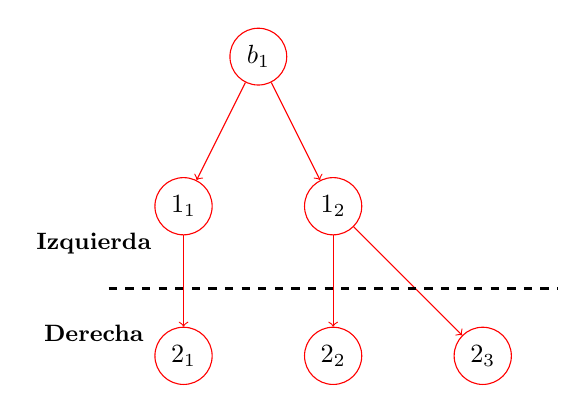
\begin{tikzpicture}[scale=.95, transform shape, 
		unrelated/.style={circle, draw=red},
		wiggly/.style={decorate, decoration={snake, amplitude=.2mm, segment length=2mm}}
		]
		
		% ---- NODOS ----
		\node[unrelated] (b1) at (0, 0) {$b_1$};
		\node[unrelated] (11) at (-1, -2) {$1_1$};
		\node[unrelated] (12) at (1, -2) {$1_2$};
		
		\node[unrelated] (21) at (-1, -4) {$2_1$};
		\node[unrelated] (22) at (1, -4) {$2_2$};
		\node[unrelated] (23) at (3, -4) {$2_3$};
		
		% ---- ARISTAS ----
		\path [->, draw=red] (b1) -- (11);
		\path [->, draw=red] (b1) -- (12);
		\path [->, draw=red] (11) -- (21);
		\path [->, draw=red] (12) -- (22);
		\path [->, draw=red] (12) -- (23);
		
		% ---- LÍNEA DE CORTE ----
		\draw[dashed, thick] (-2, -3.1) -- (4, -3.1);
		
		% ---- ETIQUETAS ----
		\node at (-2.2, -2.5) {\small \textbf{Izquierda}};
		\node at (-2.2, -3.7) {\small \textbf{Derecha}};
		
	\end{tikzpicture}
	\caption{Ejemplo de una clase de equivalencia para los nodos del subárbol de $b_1$ en la Figura \ref{fig:dtreeForestForEquivalenceClasses}, que divide los nodos en aquellos ubicados a la izquierda o a la derecha de $x_i$ en un orden topológico. En este caso la clase sería $L(\equivalenceClass) = \set{b_1, 1_1, 1_2}, R(\equivalenceClass) = \set{2_1, 2_2, 2_3}$}
	\label{fig:unrelatedSubtree}
\end{figure}


Para responder esta pregunta calculemos el número de clases de equivalencia para uno de los subárboles. Tomemos la Figura \ref{fig:unrelatedSubtree} como el subárbol $b_1$ del ejemplo anterior. Nuestro objetivo es calcular el número de clases de equivalencia del subárbol con raíz en $b_1$, $\numEqCl(b_1)$. Para $b_1$, tenemos dos opciones: puede ser posicionado a la derecha o a la izquierda de $x_i$ en el orden topológico $\toOr$. Si se posiciona a la derecha, entonces todos sus descendientes también estarán posicionados a la derecha, pues deben aparecer luego de $b_1$. Si se posiciona a la izquierda, entonces no hay ninguna restricción sobre sus descendientes. Entonces, nuestra fórmula sería:
$$\numEqCl(b_1) = \numEqCl(b_1 | \toOr(b_1) > \toOr(x_i) ) +  \numEqCl(b_1 | \toOr(b_1) < \toOr(x_i) )  = 1 + \numEqCl(b_1 | \toOr(b_1) < \toOr(x_i) ) $$

%\santi{Estaría bueno un dibujo acá contando a qué nos referimos con clase de equivalencia del árbol. Sobre el mismo dibujo podes dibujar una línea y decir que la clase queda definida por los nodos arriba de la línea y los de abajo.}

$\numEqCl(b_1 | \toOr(b_1) > \toOr(x_i) )$ lo sustituimos por 1, ya que los elementos a la izquierda de $x_i$ van a ser los mismos para todos esos órdenes topológicos, puesto que sus descendientes van a estar a la derecha, por lo que todos los órdenes topológicos con $b_1$ a la derecha van a pertenecer a la misma $\equivalenceClass$.
Ahora, si $b_1$ está posicionado a la izquierda de $x_i$, entonces no hay restricciones para sus hijos ni sus subárboles, y podemos aplicar el mismo proceso para cada uno de sus hijos. Luego, podemos combinar cada $\equivalenceClass$ obtenida en los subárboles, puesto que no tienen aristas en común. En términos de combinatoria, eso significa multiplicar el resultado que obtenemos para cada subárbol. También debemos tener en cuenta el caso en el que el nodo no tiene hijos; ahí podemos tener dos clases de equivalencia, considerando las posibilidades de izquierda y derecha. Así es como obtenemos esta fórmula:

\begin{formula}\label{formula:number_of_equiv_classes}
	Dado un nodo $n$ de un subárbol, la cantidad de clases de equivalencia con respecto a $x_i$ se calcula como:
	$$    \numEqCl(n) = 
	\begin{cases} 
		2 & \text{si $n$ es una hoja} \\
		\prod_{c \in children(n)} \numEqCl(c) + 1 & \text{oc.}
	\end{cases}
	$$
	
\end{formula}


%\santi{Sacar el ingles de la fórmula}
Esta fórmula también puede usarse para calcular las clases de equivalencia de todos los nodos \emph{no relacionados} en el ejemplo anterior. Podemos usar una estrategia similar a la utilizada para calcular los órdenes topológicos. Creamos un nodo $r_0$ y lo conectamos a las raíces de todos los subárboles de los nodos no relacionados, y luego calculamos $\numEqCl(r_0)$ utilizando la fórmula definida previamente. 

\begin{figure}[ht]
	\centering 
	\begin{tikzpicture}[scale=.95, transform shape, 
		unrelated/.style={circle, draw=red},
		wiggly/.style={decorate, decoration={snake, amplitude=.2mm, segment length=2mm}}  % Define wiggly line style
		]
		
		
		% ---- NODOS ----
		\node[nodo] (r) at (0, 0) {$r$};
		\node[nodo, draw=blue] (r0) at (4, 0) {$r_0$};
		\node[unrelated] (a1) at (-1, -2) {$a_1$};
		\node[nodo] (a2) at (1, -2) {$a_2$};
		
		\node[unrelated] (b1) at (-1, -4) {$b_1$};
		\node[nodo] (b2) at (1, -4) {$b_2$};
		\node[unrelated] (b3) at (3, -4) {$b_3$};
		
		\node[unrelated] (c1) at (0, -7) {$c_1$};
		\node[nodo] (c2) at (3, -6) {$c_2$};
		
		\node[nodo] (xi) at (3, -8) {$x_i$};
		
		
		
		\node[draw=none, fill=none] (hi) at (3, -10) {};
		
		
		\path [->] (r) edge[arista]  (a1);
		\path [->] (r) edge[arista]  (a2);
		
		\path [->] (a2) edge[arista]  (b1);
		\path [->] (a2) edge[arista]  (b2);
		\path [->] (a2) edge[arista]  (b3);
		
		\path [->] (b2) edge[arista]  (c1);
		\path [->] (b2) edge[arista]  (c2);
		
		\path [->] (c2) edge[arista]  (xi);
		
		\path [->] (r) edge[arista]  (a1);
		\path [->] (r0) edge[arista, draw=blue]  (a1);
		\path [->] (r0) edge[arista, draw=blue]  (b1);
		\path [->] (r0) edge[arista, draw=blue]  (b3);
		\path [->] (r0) edge[arista, draw=blue]  (c1);
		
		\node[text=red] at (-2, -8) {$c_1$ subtree}; 
		\draw[red, wiggly] (-1, -9) -- (0,-7.4) -- (1, -9) -- cycle;  % Draw the triangle
		
		\node[text=red] at (-3, -5) {$b_1$ subtree}; 
		\draw[red, wiggly] (-2, -6) -- (-1,-4.4) -- (0, -6) -- cycle;  % Draw the triangle
		
		\path [->] (xi) edge[arista,  decorate, decoration={snake, amplitude=.4mm, segment length=4mm, post length=1mm}] node[right] {descendants of $x_i$} (hi);
	\end{tikzpicture}
	\caption{Estrategia utilizada para calcular las clases de equivalencia de los nodos no relacionados, no de todo el DAG.}
\end{figure}

%\santi{Este párrafo biene un poco de la nada, el lector no sabe que el algoritmo tiene complejidad proporcional a las clases (o si?)}

En la sección siguiente se presenta un algoritmo para obtener las clases de equivalencia, el cual es polinomial en la cantidad de clases. Por lo que utilizando la Fórmula \ref{formula:number_of_equiv_classes}, podemos prever el tiempo que va a tomar obtener las clases de equivalencias, puesto que ya tenemos una cota para las mismas. Esta fórmula la podemos correr en tiempo polinomial para realizar una aproximación del tiempo que va a tardar. %\santi{Mejorar mucho este párrafo, la redacción esta rarísima. Hay muchos puntos.}
\begin{comment}
	Hay un caso que no estamos considerando, y es cuando los nodos no relacionados tienen ancestros. Pero ese es el mismo caso para el cual \emph{no pudimos encontrar una respuesta} en el conteo de los ordenes topológicos. En este caso, sería fácil solucionarlo, ya que solo necesitarías conectar $r_0$ a la nueva raíz del subárbol. El problema surge si el subárbol tiene múltiples raíces, entonces la fórmula que definimos anteriormente no sería suficiente, porque estaría contando algunos escenarios dos veces.    
	Al final no lo agregué, no suma tanto. 
\end{comment}

\subsection{Cota superior para las clases de equivalencia}

Queremos encontrar una cota superior para el número de clases de equivalencia de un árbol, para ver si el número de clases de equivalencia será menor que los posibles órdenes topológicos y si es que esta heurística trae consigo una mejora significativa. 

\begin{lemma}\label{lemma:upper_bound_equivalence_classes}
	Sea  $T$ un árbol con su raíz $n$, donde $l$ es el número de hojas del árbol y $h$ es su altura. Entonces, para la fórmula: 
	\[
	\numEqCl(n) = 
	\begin{cases} 
		2 & \text{if $n$ is a leaf} \\
		\prod_{c \in children(n)} \numEqCl(c) + 1 & \text{oc.}
	\end{cases}
	\]
	tenemos la cota $\numEqCl(n) \leq h^l + 1$
	
\end{lemma}

La demostración está en el apéndice en la sección \ref{subsubSection:proofUpperBoundEquivalenceClasses}. Con esta cota podemos observar que: 
\begin{itemize}
	\item Si el número de hojas es $O(\log n)$ y la altura del árbol es $O(n)$, entonces el número de clases de equivalencia está acotado por $O(n^{\log n})$. Esta cota es \emph{subexponencial}. %\santi{Esto no es exponencial. Podés decir que no es exponencial, pero tampoco polinomial (o sea, un punto medio).}, con la cota $O(n^{\log n})$. 
	\item Si la cantidad de hojas es pequeña, entonces nuestra cota va a disminuir también. Lo que significa que es mejor tener un pequeño grado de salida desde cada vértice, al igual que con los órdenes topológicos. %\santi{No me gusta nada el queremos en general. Diría directamente "Si hay pocas hojas el valor de la cota es mejor, asi que nice"}
	\item Es mejor tener una mayor altura que un grado de salida mayor con mucha ramificación.
	\item La cota para el número de clases de equivalencia depende de $h$ y $l$, a diferencia de la cota para los órdenes topológicos que solo depende de $n$, $O(n!)$. Más adelante veremos la diferencia en la práctica.
\end{itemize}
